\section{Fredo Flu}\label{fredo-flu}

Tags: Città Creatore: Davide Ispirazione: Fiumefreddo Bruzio

\section{Fredo Flu}\label{fredo-flu-1}

\begin{center}\rule{0.5\linewidth}{0.5pt}\end{center}

\begin{figure}
\centering
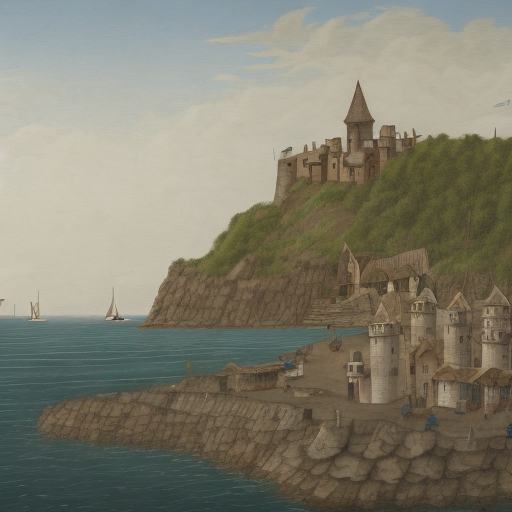
\includegraphics{a-medieval-village-by-the-sea-a-large-old-destroyed-castle-in-the-background---3.png}
\caption{a-medieval-village-by-the-sea-a-large-old-destroyed-castle-in-the-background---3.png}
\end{figure}

Informazioni Generali

Tipo di Luogo: Villaggio

Dimensioni:

Altitudine: 206 m slm

Popolazione: 258

Paese:

Luogo: Valtara

\begin{center}\rule{0.5\linewidth}{0.5pt}\end{center}

\subsection{1. Descrizione Generale}\label{descrizione-generale}

\begin{center}\rule{0.5\linewidth}{0.5pt}\end{center}

\begin{figure}
\centering
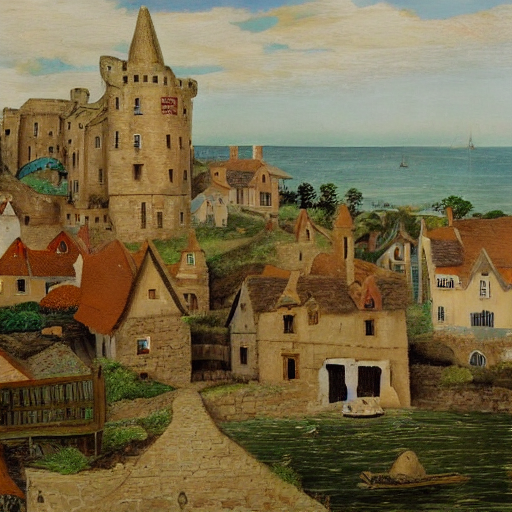
\includegraphics{a-medieval-village-by-the-sea-a-large-old-destroyed-castle-in-the-background---2.png}
\caption{a-medieval-village-by-the-sea-a-large-old-destroyed-castle-in-the-background---2.png}
\end{figure}

Fredo Flu è una città situata in un'incantevole baia circondata da
scogliere affacciate su un mare turchese. La città è caratterizzata da
un'architettura mista di costruzioni in legno e pietra, con case basse e
tetti spioventi, ed è composta principalmente da pescatori, agricoltori
e mercanti.

\begin{quote}
``Ora ti faccio una mossa di Karate'' - Frank il Barone
\end{quote}

\subsection{2. Storia}\label{storia}

\begin{center}\rule{0.5\linewidth}{0.5pt}\end{center}

La storia di Fredo Flu è profondamente radicata nella mitologia elfica.
Si racconta che la città sia stata fondata molti secoli fa da una
potente famiglia di elfi, i quali governavano su un vasto regno che si
estendeva dalle coste del mare fino alle foreste più remote. Gli elfi
hanno governato con saggezza e giustizia per molti secoli, portando
prosperità e ricchezza alla loro terra. La città di Fredo Flu era il
loro principale centro di potere e di cultura, dove si trovavano i loro
palazzi, i loro templi e le loro scuole di magia. Tuttavia, l'armonia
che regnava nel regno degli elfi venne spezzata quando una potente
maledizione colpì la famiglia regnante di Fredo Flu. Non si sa con
certezza chi abbia scagliato la maledizione, ma si dice che fosse stata
causata dall'ira degli dei a causa dell'arroganza degli elfi. La
maledizione ha causato una serie di sfortune per la famiglia degli elfi,
come la perdita della loro ricchezza, la malattia e la morte di molti
membri della famiglia. La famiglia è diventata sempre più isolata,
chiusa nella loro dimora nel palazzo reale e dimenticando lentamente la
loro posizione di potere nella città. Nel frattempo, la popolazione di
Fredo Flu ha cominciato a organizzarsi in autonomia e ad assumere un
ruolo più attivo nella gestione della città. Un sistema feudale si è
sviluppato, con un signore locale che ha preso il potere e governato con
mano dura e avarizia. La popolazione, però, non ha dimenticato il
passato glorioso della loro città e l'eredità elfica che ancora si può
vedere nei resti del palazzo reale e nelle tradizioni della città. Molte
persone sperano che un giorno la maledizione possa essere spezzata e che
gli elfi possano tornare a governare la città con la loro saggezza e il
loro potere magico.

\subsection{3. Geografia}\label{geografia}

\begin{center}\rule{0.5\linewidth}{0.5pt}\end{center}

Fredo Flu si trova su una baia incantata, circondata da scogliere e
affacciata su un mare turchese. La costa è caratterizzata da una serie
di insenature e calette nascoste, protette dalle correnti e dai venti,
che offrono un rifugio ideale per le barche dei pescatori. All'interno
del villaggio, l'architettura è basata sulle costruzioni in legno e
pietra, con case basse e tetti spioventi. Le strade sono strette e
tortuose, e sono spesso intervallate da piccole piazze o cortili
interni, dove i bambini giocano e i vecchi si rilassano al fresco. La
zona centrale del villaggio è dominata da un antico palazzo reale,
abbandonato e in rovina da secoli. Il palazzo si trova in una posizione
elevata rispetto al resto del villaggio, e offre una vista panoramica
sulla baia e sulla campagna circostante. L'edificio è stato costruito in
pietra bianca e si sviluppa su tre piani, con un cortile interno
circondato da colonne e archi. Alle spalle del villaggio si estende una
vasta foresta, che ospita creature magiche e pericolose, come i folletti
e i lupi mannari. La foresta è attraversata da un fiume che scorre verso
il mare, e che offre un'abbondante risorsa di pesce e di acqua dolce.
Inoltre, il mare intorno al villaggio è abitato da creature misteriose e
pericolose, come sirene e kraken, che rendono la pesca un'attività
rischiosa e avventurosa. Tuttavia, i pescatori del villaggio devono
affrontare ogni giorno la sfida di catturare abbastanza pesce senza
essere attaccati dalle creature del mare. In generale, il paesaggio
circostante Fredo Flu è caratterizzato da colline verdi e morbide,
punteggiate da campi coltivati e boschi. La regione è famosa per la sua
natura incontaminata e selvaggia, e attira molti visitatori che vogliono
godere della bellezza del luogo e della sua pace rilassante.

\subsubsection{3.1 Distretti}\label{distretti}

Il villaggio di Fredo Flu è diviso in 3 quartieri:

\begin{enumerate}
\def\labelenumi{\arabic{enumi}.}
\tightlist
\item
  \textbf{Marina:} è la zona residenziale. Qui abita la maggior parte
  della popolazione di Fredo Flu. È caratterizzata da colorate case in
  legno e piccole botteghe.
\item
  \textbf{Paisi:} è la zona abitata dall'attuale nobiltà. Ciò che resta
  del palazzo reale è la residenza estiva della famiglia nobiliare.
\item
  \textbf{Santuiasi:} è la zona più rurale di Fredo Flu. Qui vive gente
  poco raccomandabile, a cui piace viaggiare su carri rumorosi e con
  vari ornamenti a vista, come ad esempio la tipica zampa di lepre o
  coda di volpe appesi in giro per il carro.
\end{enumerate}

\subsection{4. Demografia}\label{demografia}

\begin{center}\rule{0.5\linewidth}{0.5pt}\end{center}

Fredo Flu è un villaggio di medie dimensioni con una popolazione
variegata e multietnica. La maggior parte degli abitanti sono umani, sia
di origine locale che provenienti da altri villaggi o città vicine.
Tuttavia, c'è anche una significativa popolazione elfica, che vive
principalmente nel quartiere del Palazzo. Questi elfi sono noti per la
loro eleganza e la loro raffinatezza, anche se negli ultimi tempi hanno
perso gran parte della loro ricchezza e del loro potere a causa della
maledizione che ha colpito la loro famiglia. Oltre agli umani e agli
elfi, ci sono anche altre creature che abitano il villaggio, come gnomi,
nani e mezzelfi, che sono presenti in minor numero. Queste creature sono
conosciute per la loro abilità artigianale e spesso gestiscono piccole
botteghe nel quartiere della Marina. La popolazione di Fredo Flu è
principalmente di fede religiosa, con una forte devozione per il culto
degli antenati elfici. Ci sono vari templi e santuari dedicati agli dei
elfici, come il dio della natura e della caccia, che sono spesso
visitati dagli abitanti del villaggio durante le feste religiose. In
termini di occupazioni, la maggior parte degli abitanti del villaggio si
dedicano all'agricoltura e alla pesca, grazie alla posizione favorevole
del villaggio sulla costa. Ci sono anche alcuni artigiani e commercianti
che gestiscono negozi nel centro del villaggio, così come alcuni guardie
e soldati che si occupano della sicurezza e della difesa del villaggio.
Nel complesso, Fredo Flu è una comunità multietnica e multiculturale,
con una ricca storia e tradizioni che si mescolano tra umani ed elfi.

\subsection{6. Cultura}\label{cultura}

\begin{center}\rule{0.5\linewidth}{0.5pt}\end{center}

La cultura di Fredo Flu è fortemente influenzata dalla sua antica storia
elfica, e gli abitanti del villaggio hanno un grande rispetto e una
forte venerazione per la società elfica del passato. La leggenda narra
che il villaggio fosse una volta la capitale di un grande regno elfico,
governato dalla nobile famiglia che ora vive nel palazzo reale. Gli
abitanti di Fredo Flu sono molto fieri della loro eredità elfica e
cercano di preservare le tradizioni e le usanze di questo popolo antico.
Le festività tradizionali del villaggio riflettono l'influenza
dell'eredità elfica. Durante la festa di San Rock-Oh, ad esempio, gli
abitanti del villaggio si vestono con abiti tradizionali ispirati alla
moda elfica e celebrano con canti e balli che richiamano la cultura
elfica. Durante la festa di Yule, invece, gli abitanti del villaggio
decorano le case e le strade con luci e ornamenti ispirati al periodo
elfico di prosperità e magia. L'arte e la musica di Fredo Flu sono anche
molto influenzate dalla cultura elfica. La musica tradizionale del
villaggio include strumenti come il flauto, la lira e il violino, che
ricordano gli strumenti usati dagli elfi nella loro musica. Le opere
d'arte locali includono spesso immagini di creature magiche e paesaggi
fantastici, e sono create con tecniche che richiamano le tecniche di
pittura e scultura elfiche. In sintesi, la cultura di Fredo Flu è un mix
di influenze elfiche e umane, che creano un mondo fantastico e magico.
La venerazione dell'antica società elfica è una parte importante della
cultura del villaggio, e la sua celebrazione è un modo per gli abitanti
di mantenere viva la memoria di un passato glorioso.

\subsubsection{6.1 Cucina}\label{cucina}

\begin{center}\rule{0.5\linewidth}{0.5pt}\end{center}

La cucina di Fredo Flu è un'altra manifestazione della cultura del
villaggio. Le ricette tradizionali riflettono l'influenza
dell'entroterra e del mare, ma sono preparate con tecniche che
richiamano i sapori e le tradizioni culinarie dell'antica società
elfica. Ad esempio, alcuni piatti includono ingredienti magici come le
bacche elfiche o il succo di mele di Yggdrasil, che si dice abbiano
proprietà curative e magiche.

\subsection{7. Governo}\label{governo}

\begin{center}\rule{0.5\linewidth}{0.5pt}\end{center}

La forma di governo di Fredo Flu è quella di un sistema feudale, con un
signore locale che governa sulla popolazione. Il signore, noto per la
sua crudeltà e la sua avarizia, esercita il suo potere attraverso una
serie di funzionari e ufficiali che agiscono a suo nome. Il signore ha
il controllo completo sull'esercito e sulla giustizia locale. La
popolazione non ha alcun potere decisionale e non ha voce in capitolo
sulle questioni che riguardano il villaggio. Nonostante ciò, ci sono
alcune famiglie nobili che godono di un certo livello di autonomia e
rispetto dal signore. In particolare, la famiglia degli elfi nobili che
risiede nel palazzo reale ha una certa influenza nella vita del
villaggio, anche se ultimamente hanno perso gran parte della loro
ricchezza e del loro potere a causa della maledizione che li ha colpiti.
In generale, il governo di Fredo Flu è caratterizzato da una forte
oppressione e ingiustizia, con la popolazione costretta a sopportare le
conseguenze delle decisioni del signore locale senza avere alcun diritto
di protestare o di cambiare la situazione.

\subsection{8. Persone famose}\label{persone-famose}

\begin{center}\rule{0.5\linewidth}{0.5pt}\end{center}

\begin{itemize}
\tightlist
\item
  \textbf{San Rock-Oh}: Elfo che in passato regnava su Fredo Flu. Molte
  storie della città narrano le sue imprese che portarono il paese ad
  essere uno dei fulcri della regione. Purtroppo le fonti storiche sono
  andate perse e spesso leggenda e realtà si mischiano.
\item
  \textbf{Rhino}: Viandante che passa spesso dal villaggio. Nessuno sa
  cosa faccia nella vita, ma ci sono storie di secoli fa che parlano di
  lui. Che sia immortale?
\item
  \textbf{Frank il Barone}: Vecchio gnomo ubriacone. Racconta spesso
  delle sue avventure immaginarie in cui combatte con mostri
  giganteschi. Secondo la sua versione lui ha 7 mogli sparse per le 7
  maggiori città di Valtara e con ognuna ha 7 figli. Nessuno gli crede.
\end{itemize}
